\documentclass{article}

\usepackage{graphicx}
\usepackage{tikz}
\usepackage{tikzsymbols}
\usetikzlibrary{calc,patterns,shapes.geometric}
\pagestyle{empty}

\def\centerarc[#1](#2)(#3:#4:#5){\draw[#1] ($(#2)+({#5*cos(#3)},{#5*sin(#3)})$) arc (#3:#4:#5);}

\begin{document}
	\centering
	\begin{figure}
			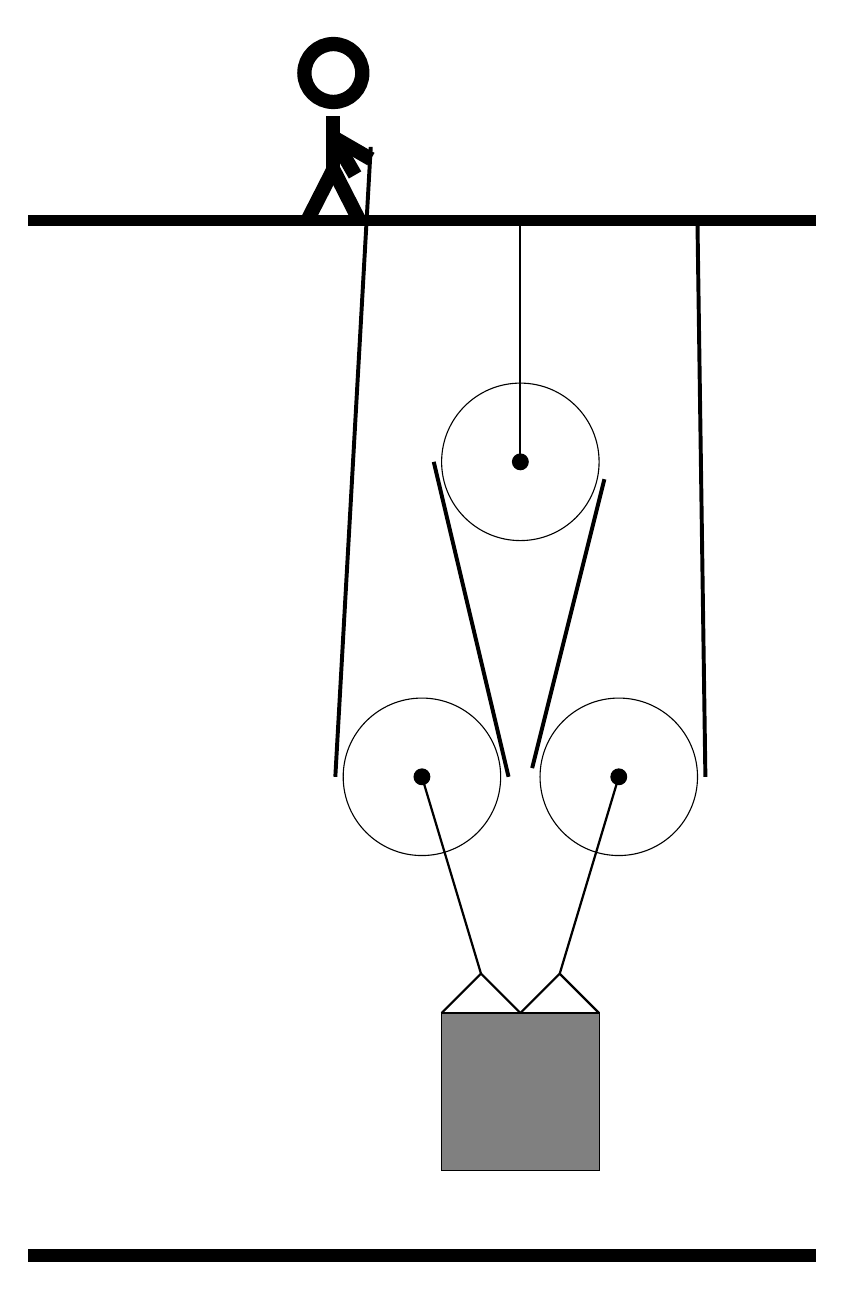
\begin{tikzpicture}
				%%%%% START %%%%%
								\draw[fill=black] (-4, 10) rectangle (6, 10.125);
				
				\draw (1, 3.0) circle (1);
				\draw[fill=black] (1, 3.0) circle (0.1);
				
				\draw (2.25, 7.0) circle (1);
				\draw[fill=black] (2.25, 7.0) circle (0.1);
				\draw[thick] (2.25, 7.0) -- (2.25, 10);
				
				\draw (3.5, 3.0) circle (1);
				\draw[fill=black] (3.5, 3.0) circle (0.1);
				
				\draw[thick] (3.5, 3.0) -- (2.75, 0.5);
				\draw[thick] (1, 3.0) -- (1.75, 0.5);
				\draw[thick]  (1.25, 0) -- (1.75, 0.5) -- (2.25, 0);
				\draw[thick]  (2.25, 0) -- (2.75, 0.5) -- (3.25, 0);
				\draw[fill=black!50] (1.25, 0) rectangle (3.25, -2);
				
				\draw[line width=0.5mm] (0.35, 11) --  (-0.1, 3.0);
				\centerarc[line width=0.5mm](1, 3.0)(180:360:1.1);
				\draw[line width=0.5mm] (2.1, 3.0) -- (1.15, 7.0);
				\centerarc[line width=0.5mm](2.25, 7.0)(-20:180:1.1);
				\draw[line width=0.5mm](3.317, 6.78) -- (2.4, 3.11);
				\centerarc[line width=0.5mm](3.5, 3.0)(160:360:1.1);
				\draw[line width=0.5mm](4.6, 3.0) -- (4.5, 10);
				
				\node at (-0.07, 11.2) {\Strichmaxerl[10][120][-30]};
				
				\draw[fill=black] (-4, -3) rectangle (6, -3.15);
				%%%%% END %%%%%
			\end{tikzpicture}
	\end{figure}	
\end{document}